
\documentclass[12pt, a4paper, oneside, headinclude, footinclude]{article}

%----------------------------------------------------------------------------------------
%	REQUIRED PACKAGES
%----------------------------------------------------------------------------------------

\usepackage[
nochapters, 
beramono, 
eulermath,
pdfspacing, 
dottedtoc 
]{classicthesis} 

\usepackage{arsclassica} 
\usepackage{listings} 
\usepackage{minted} 
\usepackage[T1]{fontenc} 
\usepackage[utf8]{inputenc} 
\usepackage{graphicx} 
\graphicspath{{Figures/}} 
\usepackage{enumitem} 
\usepackage{lipsum} 
\usepackage{subfig} 
\usepackage{amsmath,amssymb,amsthm} 
\usepackage{varioref} 

%----------------------------------------------------------------------------------------
%	THEOREM STYLES
%---------------------------------------------------------------------------------------

\theoremstyle{definition} 
\newtheorem{definition}{Definition}

\theoremstyle{plain} 
\newtheorem{theorem}{Theorem}

\theoremstyle{remark} 

%----------------------------------------------------------------------------------------
%	HYPERLINKS
%---------------------------------------------------------------------------------------

\hypersetup{
colorlinks=true, breaklinks=true, bookmarks=true,bookmarksnumbered,
urlcolor=webbrown, linkcolor=RoyalBlue, citecolor=webgreen, 
pdftitle={}, 
pdfauthor={\textcopyright}, 
pdfsubject={}, 
pdfkeywords={}, 
pdfcreator={pdfLaTeX}, 
pdfproducer={LaTeX with hyperref and ClassicThesis} 
}


\title{\normalfont\spacedallcaps{Image analysis for disaster recovery, A DataKind report for the World Bank GFDRR}}

\author{\spacedlowsmallcaps{Krishna Bhogaonker \& Patrick Doupe}} 

\date{} 

\begin{document}

\renewcommand{\sectionmark}[1]{\markright{\spacedlowsmallcaps{#1}}} 
\lehead{\mbox{\llap{\small\thepage\kern1em\color{halfgray} \vline}\color{halfgray}\hspace{0.5em}\rightmark\hfil}} 

\pagestyle{scrheadings} 

%----------------------------------------------------------------------------------------
%	TABLE OF CONTENTS & LISTS OF FIGURES AND TABLES
%----------------------------------------------------------------------------------------

\maketitle 

\setcounter{tocdepth}{2}

\tableofcontents 

\listoffigures 

\listoftables

%----------------------------------------------------------------------------------------
%	ABSTRACT
%----------------------------------------------------------------------------------------

\section*{Abstract}

We discuss how the World Bank can use machine learning and satellite images to
improve disaster relief efforts. We include a review of image analysis with
convolutional neural networks. These networks are illustrated with code
examples using the Keras deep learning library. 

%----------------------------------------------------------------------------------------
%	AUTHOR AFFILIATIONS
%----------------------------------------------------------------------------------------

%\let\thefootnote\relax\footnotetext{* \textit{}}

%\let\thefootnote\relax\footnotetext{\textsuperscript{1} \textit{}}

%----------------------------------------------------------------------------------------

\newpage 

%----------------------------------------------------------------------------------------
%	INTRODUCTION
%----------------------------------------------------------------------------------------

\section{Introduction}

The review of deep learning~\cite{lecun2015deep}.

\subsection{Terms of reference or questions to be answered}

\subsection{Main recommendations}


%----------------------------------------------------------------------------------------
%	METHODS
%----------------------------------------------------------------------------------------

\section{Frameworks}

If we present methods, it would be good to introduce frameworks up front.

\subsection{Keras}


\begin{minted}{python}
from keras.layers import Input
from keras.layers import Dense
from keras.models import Model

# This returns a tensor
inputs = Input(shape=(10,))
predictions = Dense(1, activation='softmax')(inputs)
model = Model(inputs=inputs, outputs=predictions)
model.compile(optimizer='rmsprop',
              loss='categorical_crossentropy',
              metrics=['accuracy'])
# starts training
model.fit(data, labels)  
\end{minted}



\subsection{Tensorflow, PyTorch, Caffe, MXNet, etc.}

Links to sites and  blog articles

\section{Methods}

\subsection{Why convolutional neural networks}

1. Pixels are not independent of one another
2. With pictures, only relative position matters [Spatially stationary
statistics]
3. Much fewer neurons.

Results of image analysis

\subsubsection{If you understand VGG-net, you're 80 per cent there}

VGG net is super simple and easy to explain.

\section{Literature}

\subsection{Image classification}

LeNet

Krizhevsky ImageNet~\cite{NIPS2012_4824}
\begin{itemize}
    \item Used dropout to prevent overfitting
    \item We start to go deep: 5 convolutional layers
    \item Got best results to that date on a hard problem
\end{itemize}


VGG Net~\cite{SimonyanZ14a}
\begin{itemize}
    \item Increased depth (16--19 layers) with smaller filters
    \item First/Second places at ImageNet2014
    \item Widely used as a base: need references.
\end{itemize}

ResNet~\cite{he2016deep}

\begin{itemize}
    \item Residual learning framework
    \item Degradation became an issue with deep models. This makes no sense,
        you could just have a shallower model with identity mappings. So
        residual networks contain the identity mapping.
    \item Crazy large: 152 layers but with lower `complexity'
    \item Then state of the art.
\end{itemize}

\subsection{Object detection}

Classification + localising objects. The challenge: ``detect a \textit{potentially large
number of object instances with varying sizes in the same image} using a
limited amount of computing resources.''~\cite[Their emphasis]{NIPS2013_5207}

Super basic model: slide a classifier across an image. This will be very slow.

Potentially
useful~\url{https://towardsdatascience.com/object-detection-with-10-lines-of-code-d6cb4d86f606}

\textbf{Using regression to do this}~\cite{NIPS2013_5207}

The DNN based regression outputs a binary mask of the bounding box. 

Seven layer network: five convolutional and two fully connected. ReLU and max
pooling. Note that output much smaller than input.

Instead of a softmax, they have a regression layer that outputs a binary mask:
1 if image inside the box, 0 outside.\ 

p. 3 Because base network highly non convex -> no guarantee for optimal solution ->
regularisation.

Regularisation: objects are small relative to image size, so an output of all
0s is super common. Use regularisation to increase weights of non zero
outputs.

Have five networks: one for box predictions, four others for {top, bottom,
left, right}. 
It is possible to share layers. 

Since output smaller than inputs, need to upscale

The details regarding refinement etc are a little confusing. 

Training: model needs to be trained with a huge amount of training data:
objects of different sizes need to occur at almost every location. << is this
an issue for satellite monitoring?

Pre training on classification task used.

Need to train a single model per object type and mask type.

Doesn't work super well: mAP = 30.5\%

\textbf{RCNN}~\cite{Girshick2014, Girshick2015}

Regions with CNN features
Improved on mAP (mean Average Precision) by more than 30\%. They get mAP of
53.3\%. 

Idea
\begin{enumerate}
    \item extract some 2k bounding boxes (region proposals)
    \item warp boxes and run through CNN and SVM to classify
\end{enumerate}

Use `recognition using regions' paradigm.
Alternatives: Regression like above, sliding windows.

A challenge --- labelled data is scarce. Common answer is to do unsupervised
pre training followed by supervised fine tuning. They also use supervised pre
training on a large dataset.

There are many options for proposing regions, RCNN uses `selective-search'
They also use VGG net for features.

RCNN is multi stage, expensive and s l o w. `R-CNN is slow because it performs
a ConvNet forward pass for each object proposal, without sharing computation.
(fast RCNN paper)'

\textbf{Fast-RCNN} single stage training algorithm. 

Spatial Pyramid Pooling Networks (SPPnets). SPPnets compute a feature map
for image, classifies each object proposal using shared features. But this is
a multi stage pipeline.

Multi task loss function
    (a) classification
    (b) 4d regression for bounding box

It's faster than SPPnet/RCNN but there is still a bottle neck of region
proposals

Use a single network for feature extraction, classification and bounding box.


\textbf{Faster RCNN}~\cite{Ren2017}

Because of proposal bottleneck: they propose a `Region Proposal Network.' RPNs
share layers with the object detection networks --- this allows a speed up.
E.g.\ from 2 or 0.2s per image to 10ms per image.

The RPN is basically (?) an attention network.

RPN takes anchors and (1) is this an object (2) can we adjust the anchor box
a little to get better fit (rather than absolute corners, predict change from
anchor box corners).

FasterRCNN is trainable end to end.

So at the end you get a set of overlapping proposals. If we have two
overlapping images, discard one with lower classification score.

\url{https://tryolabs.com/blog/2018/01/18/faster-r-cnn-down-the-rabbit-hole-of-modern-object-detection/}
Predicing (xmin, xmax, ymin, ymax) is hard. For instance, how to enforce
xmin < xmax

Potential code:
\url{https://github.com/jinfagang/keras\_frcnn/blob/master/keras\_frcnn/vgg.py}

Useful overview:
\url{https://blog.athelas.com/a-brief-history-of-cnns-in-image-segmentation-from-r-cnn-to-mask-r-cnn-34ea83205de4}

\textbf{Mask RCNN}~\cite{he2017}

We can do segmentation as well! Have a third branch that allows segmentation. 

But there is a slight misalignment between bounding boxes and pixels because
of pixel integers. The original image is say 200 $\times$ 200 and the feature map is
say 30 * 30. So to select the top 15*15 corner we need 15 * 30 / 200 $\approx$
2.25 pixels. RoIPool uses 2$\times$2. RoIAlign (this paper's innovation) uses
bilinear interpolation to get an idea of what the 2.25th pixel is.


\textbf{R-FCN}~\cite{NIPS2016_6465}

The above apply a costly per region subnetwork hundreds of times :(

\textit{Translation invariance} - the object can be anywhere in an image for
correct classification

\textit{Translation variance} - if we move the object, the bounding box should
change. 

Use an RPN for proposals.

\textbf{YOLO}~\cite{redmon2016yolo}

\url{http://www.youtube.com/watch?v=NM6lrxy0bxs}

YOLO is super fast. Not most accurate tho. Might be useful for large satellite
areas.

YOLO generalises to new domains (e.g. art)

Divide image into S $\times$ S grid. 
For each grid, 
    1. have B bounding boxes. 
    For each bounding box, 
        predict 5 components (4 spatial {x, y, w, h}, 1 confidence). 
        (x, y) -- center of the box relative to the bounds of the grid cell. 
        (w, h) -- width and height relative to whole image
        confidenc -- IOU between predicted and ground truth.
    2. Predict C conditional class probabilities
       Prob(Class | Object)
       Only one set of class probabilities regardless of the number of boxes
       B.

At test time: the confidence * class probabilities for class specific
confidence scores for each box.

Use Google LeNet.

Limitations: 
1. strong spatial constraints -- hard coded grid size and number of
bounding boxes and classes per box. Many small birds will be hard to predict.
--- also houses ---

2. struggles to generalise to objects with new aspect ratios. so will want a
variety of house angles. may be difficult to work with damaged buildings 

YOLO v2: big step was using imagenet and backproping classification on this
data

\textbf{SSD}~\cite{liu2016ssd}

Similar to YOLO but use multiple feature maps (grid sizes). Faster, Stronger
than YOLO v1.

\subsection{Image segmentation}

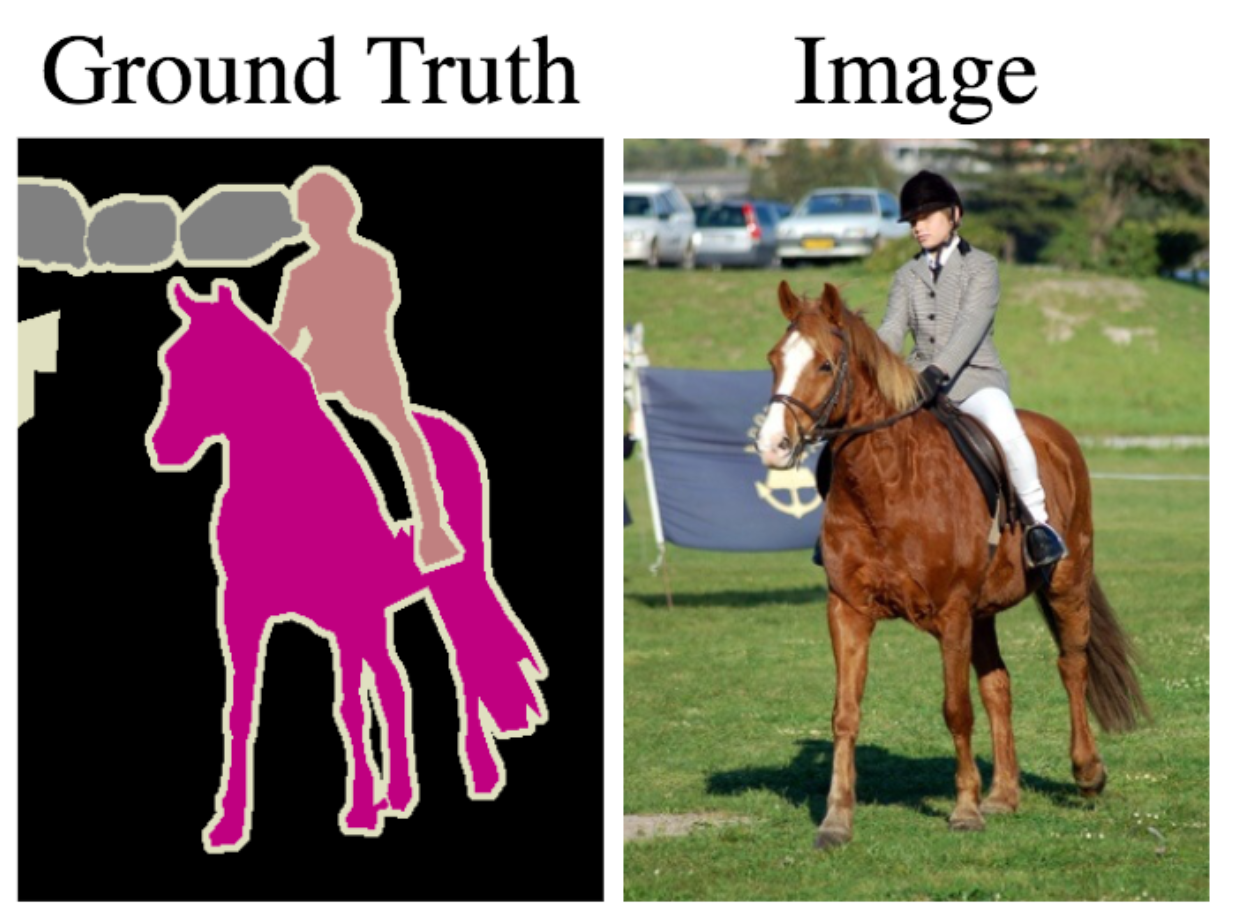
\includegraphics[width=0.5\textwidth]{Figures/segmentation-example.png}

In one sense this is a simple extension of classification: but one prediction
per pixel rather than one prediction per picture.

With segmenation, there is a tension between `semantics and location.'
\textit{Semantics} is the question of what, \textit{location} asks where.
Local information helps answer the former and global information helps answer
the latter. This need for two types of information gave rise to complicated
models prior to the era of fully end to end differentiable models. This
tension also explains the innovations beyond basic CNNs used for
classification.

Old methods: classifier applied to each object location and scale.
See~\cite{NIPS2015_5852}.

\paragraph{First fully convnet (trained end to end) segmenter}

BTW, very good write up on convnets.~\cite{long2015fully}

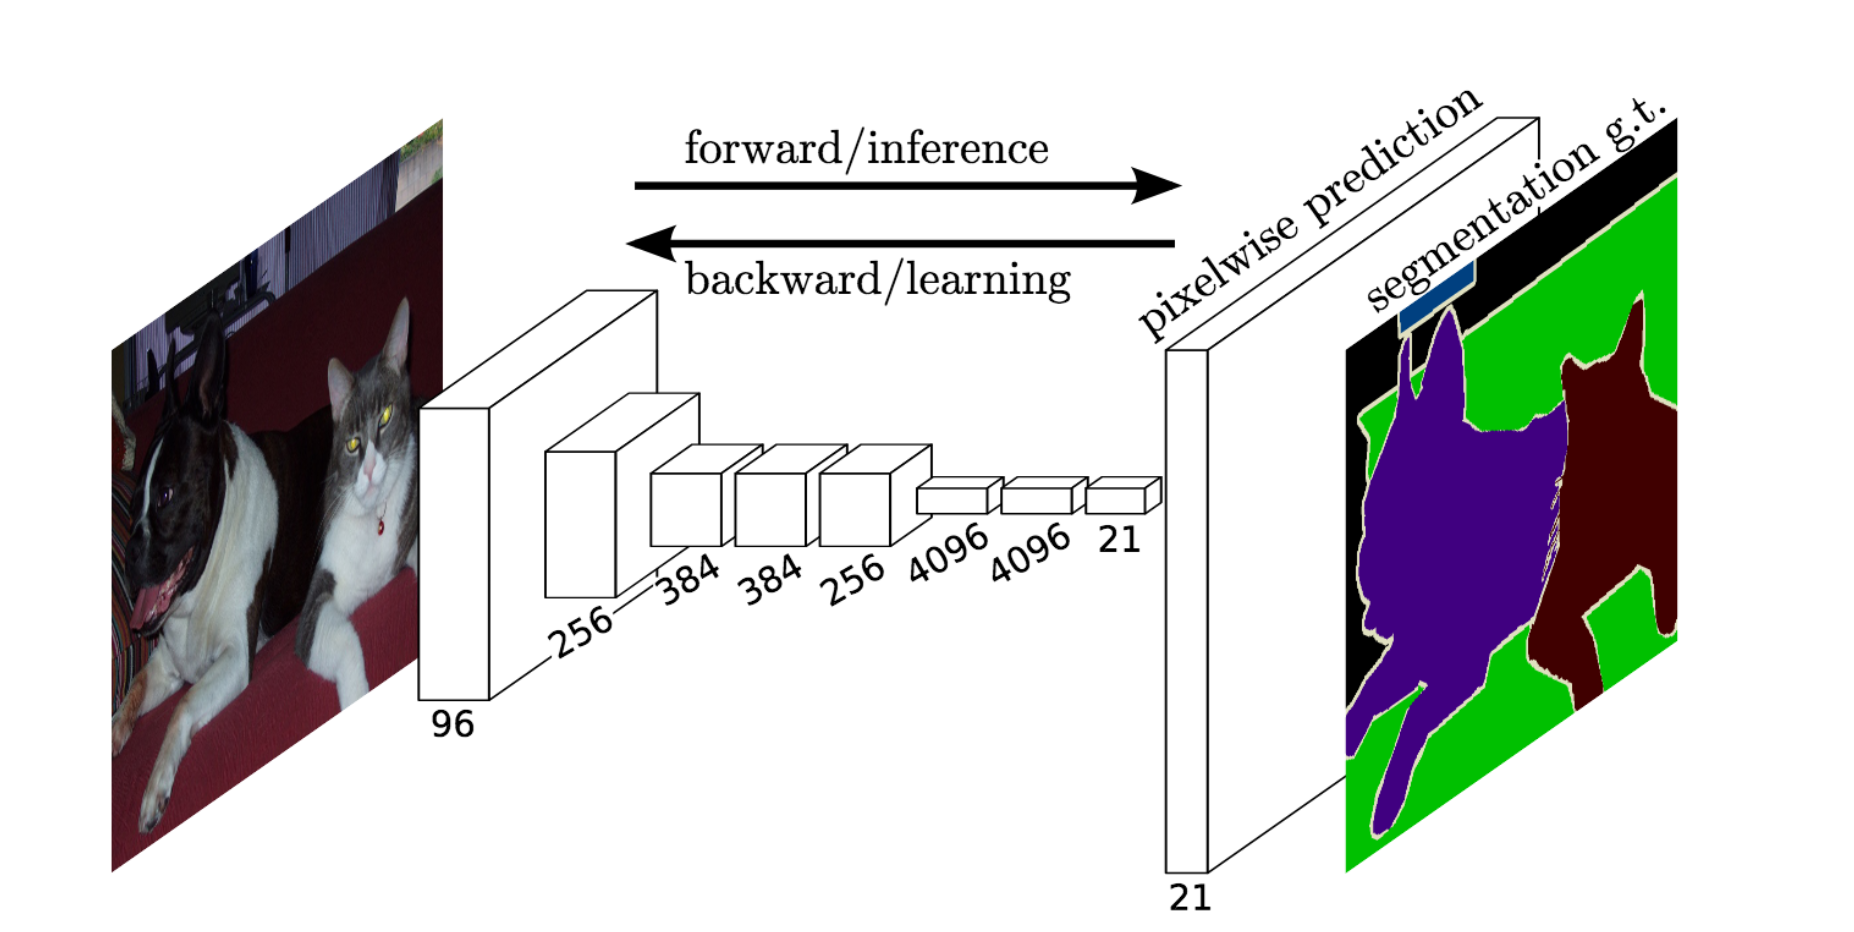
\includegraphics[width=0.5\textwidth]{Figures/long-segmentation.png}
\begin{itemize}
    \item uses in network upsampling
    \item doesn't require complicated chaining of pieces
    \item can use pre trained models
    \item use a skip architecture to combine coarse semantic information and shallow
appearance information.
\end{itemize}
There is a super easy way to make a simple CNN classifier a segmenter: make
the fully connected layers have a different height and width for each of the
4096 components.

An issue: by the time you've gotten to predicting a pixel, you've lost a lot
of the information on the surrounding pixels. The authors get around this by
bringing intermediate layers back into the prediction.

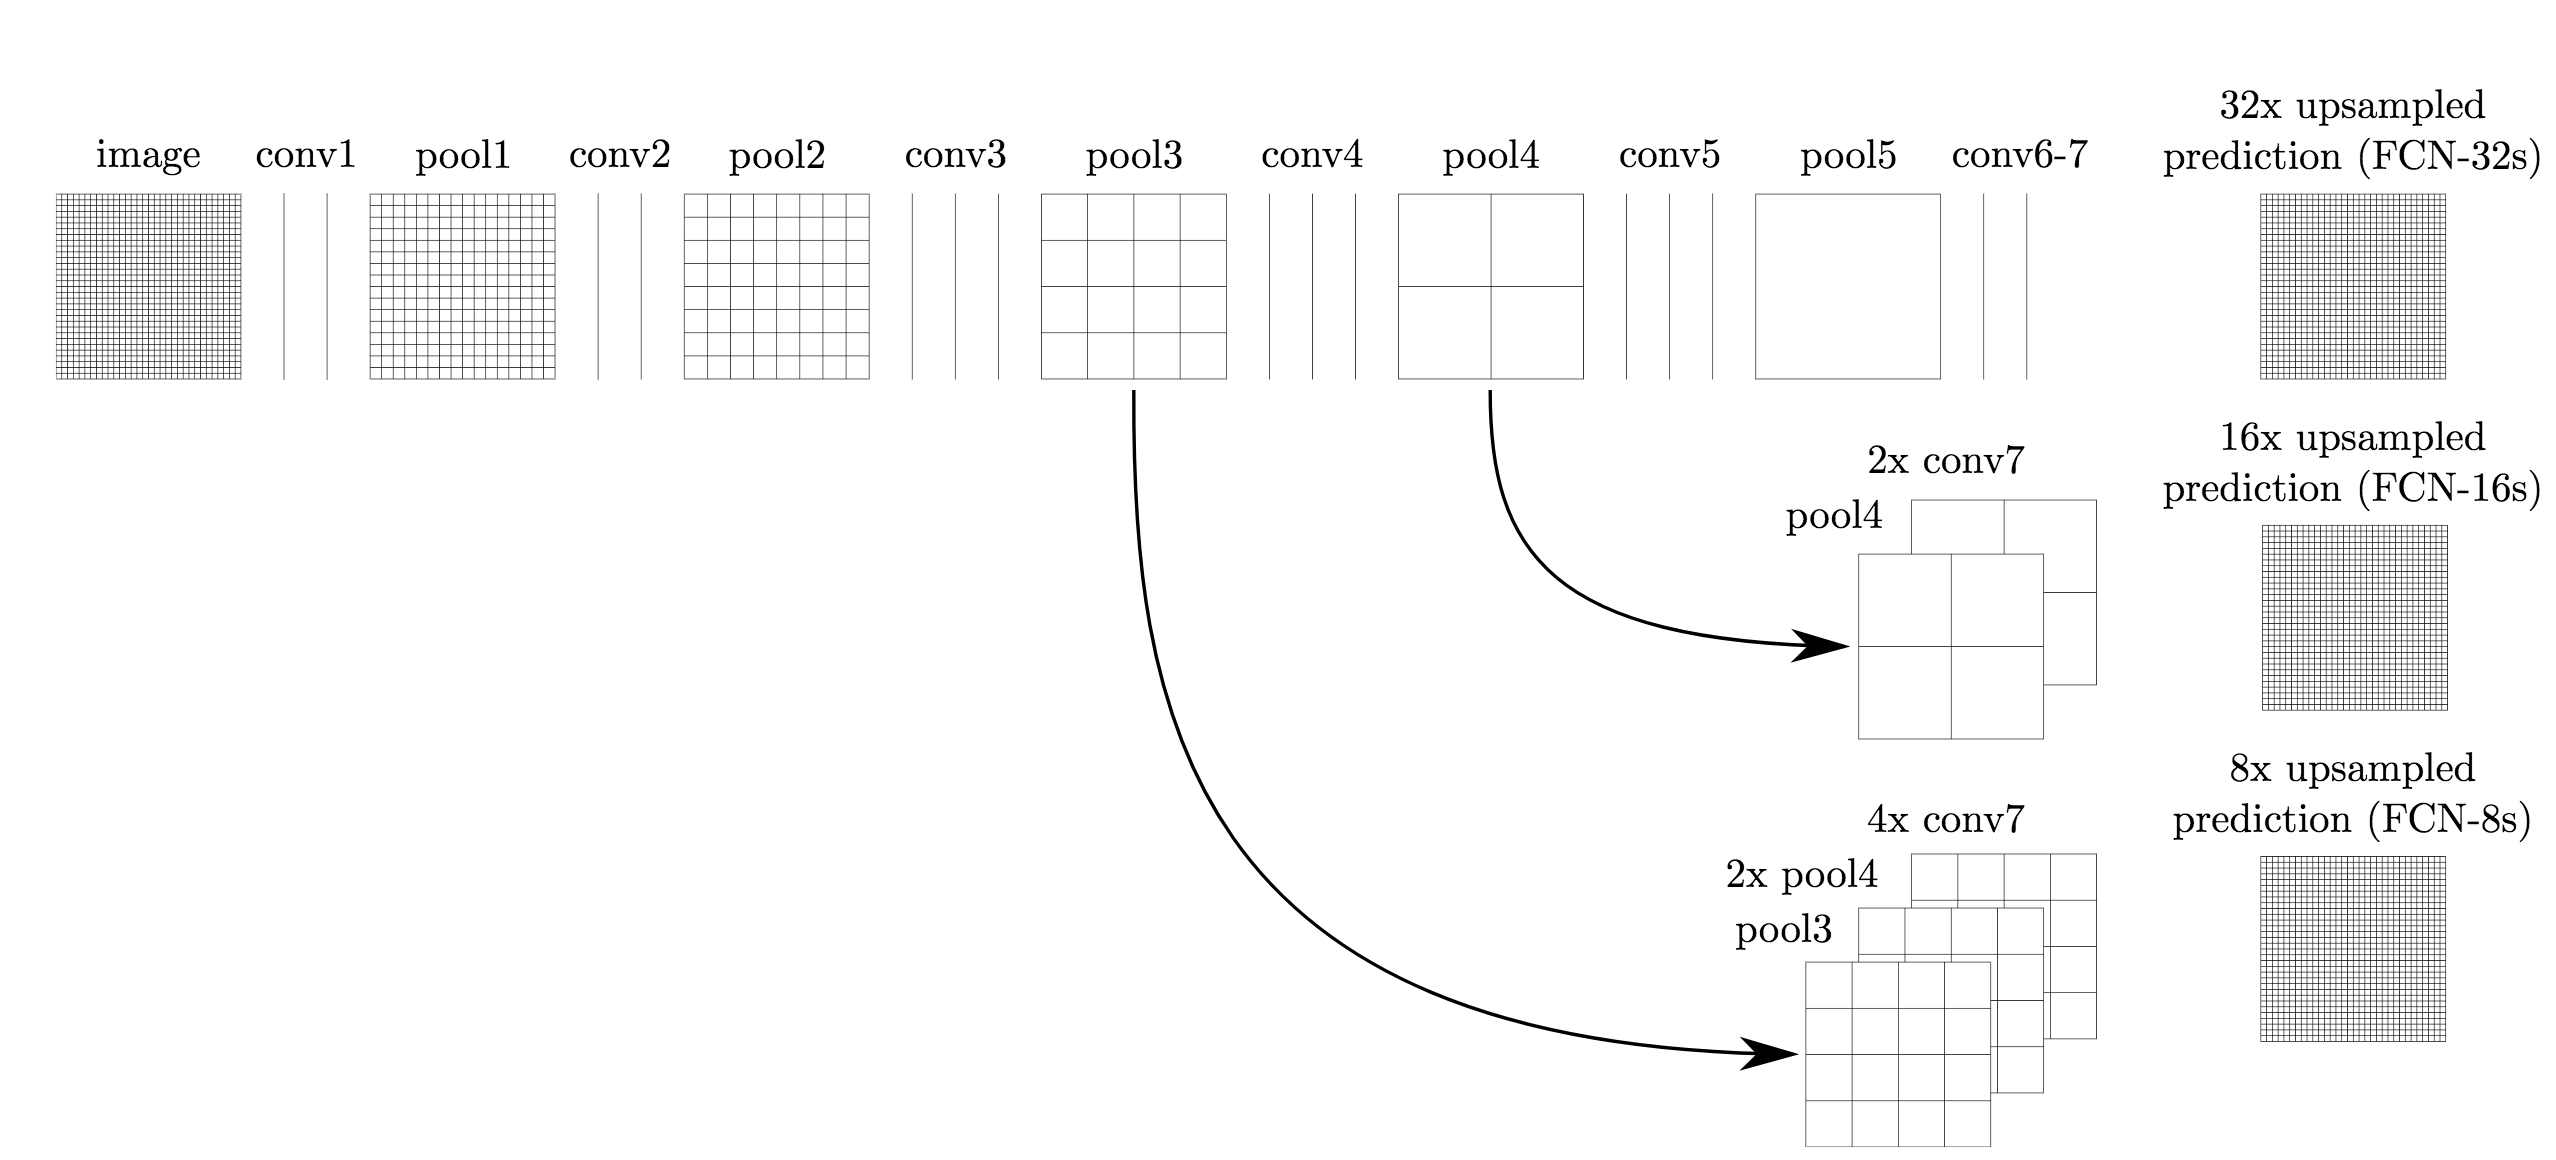
\includegraphics[width=0.75\textwidth]{Figures/skip-segmentation.png}

Some more~\cite{chen2018, NIPS2015_5852}

\paragraph{DeepLab}~\cite{chen2018}

\begin{itemize}
    \item convolution with upsampled filters --- allows control of resolution
        (or the context without increasing the number of parameters)
    \item spatial pyramid pooling: segment at multiple scales
    \item use conditional random fields to improve location accuracy (max
        pooling and down sampling lower locational accuracy)
\end{itemize}

They do this upsampling \textit{algorithme a trous} thing that~\cite{NIPS2015_5852}
do (i think).

\paragraph{Learning to segment object candidates}~\cite{NIPS2015_5852}

A model trained with two objectives
A convnet that branches out into two objecives.

\begin{enumerate}
    \item given an image patch ---  output a class agnostic segmentation mask
    \item the likelihood of the patch being centered on a full object
\end{enumerate}

Model generalizes to unseen categories it has not seen during training. Strong
work.



\subsection{Analysis with satellite images}

Mexico~\cite{babenko2017poverty} (There are two WB co-authors)

Poverty mapping~\cite{Jean790}

Population~\cite{doupe2016, robinson2017}

Private sector~\cite{facebook, cnn_orbital}

\section{Satellite data}

Planet Labs: \url{https://www.planet.com/}
Planet Labs free datasets:
~\url{https://www.planet.com/disasterdata/datasets/}
    ``We provide limited access to Explorer for up to 30 days to qualified disaster
    volunteer organizations, humanitarian organizations, and other coordinating
    bodies.''
3-5 meter imagery anywhere in the world. This may be too large for small
buildings.

**Insurance companies do this** ~~ Planet labs e book.
Predicting claim amounts // categorize unaffected assets, damaged or requiring
assessor // 
Nice image of water damage. I believe there is a way of measuring this from
space.

Satellogic has images with 30 bands. And are open for humanitarian efforts. ~\url{https://www.satellogic.com/commitment-to-science}

TellusLabs do crop monitoring and forecasting. VanderSat also on land use

Spaceknow can spot cars, buildings, etc
~\url{https://www.spaceknow.com/satellite-ai/}

Quasi free: Bing

\subsection{Expensive sources}

Digital Globe, Planet Labs, Own drone data

\subsection{Labelled data}

\subsection{Augmentation}

Talk about data augmentation. For example, U-Net used this.

\section{Examples}

\subsection{Building detection}

\section{Recommendations}

%----------------------------------------------------------------------------------------
%	BIBLIOGRAPHY
%----------------------------------------------------------------------------------------

\renewcommand{\refname}{\spacedlowsmallcaps{References}} 

\bibliographystyle{unsrt}

\bibliography{review.bib}

%----------------------------------------------------------------------------------------

\end{document}
